% The degenerate conic ^2-y^2=0$, a union of two lines.
% Source: book/tex/riemann-surface/affine-projective.tex (§ Reducible varieties).
\documentclass[border=2mm]{standalone}
\usepackage{tikz}
\usepackage{amssymb}
\usetikzlibrary{arrows.meta}
\begin{document}
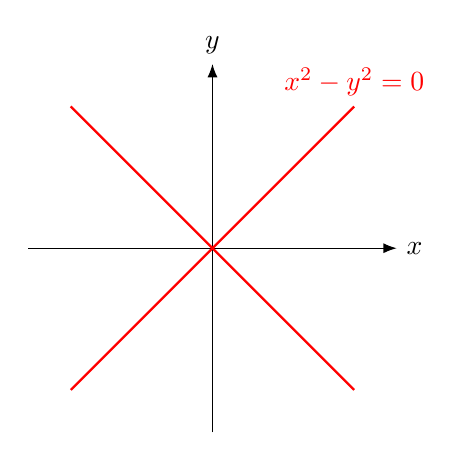
\begin{tikzpicture}[>=Latex,scale=0.9]
\draw[->](-2.6,0)--(2.6,0)node[right]{$x$};\draw[->](0,-2.6)--(0,2.6)node[above]{$y$};
\draw[red,thick](-2,-2)--(2,2)node[above]{$x^2-y^2=0$};\draw[red,thick](-2,2)--(2,-2);
\end{tikzpicture}
\end{document}
